\documentclass[twoside]{book}

% Packages required by doxygen
\usepackage{fixltx2e}
\usepackage{calc}
\usepackage{doxygen}
\usepackage[export]{adjustbox} % also loads graphicx
\usepackage{graphicx}
\usepackage[utf8]{inputenc}
\usepackage{makeidx}
\usepackage{multicol}
\usepackage{multirow}
\PassOptionsToPackage{warn}{textcomp}
\usepackage{textcomp}
\usepackage[nointegrals]{wasysym}
\usepackage[table]{xcolor}

% Font selection
\usepackage[T1]{fontenc}
\usepackage[scaled=.90]{helvet}
\usepackage{courier}
\usepackage{amssymb}
\usepackage{sectsty}
\renewcommand{\familydefault}{\sfdefault}
\allsectionsfont{%
  \fontseries{bc}\selectfont%
  \color{darkgray}%
}
\renewcommand{\DoxyLabelFont}{%
  \fontseries{bc}\selectfont%
  \color{darkgray}%
}
\newcommand{\+}{\discretionary{\mbox{\scriptsize$\hookleftarrow$}}{}{}}

% Page & text layout
\usepackage{geometry}
\geometry{%
  a4paper,%
  top=2.5cm,%
  bottom=2.5cm,%
  left=2.5cm,%
  right=2.5cm%
}
\tolerance=750
\hfuzz=15pt
\hbadness=750
\setlength{\emergencystretch}{15pt}
\setlength{\parindent}{0cm}
\setlength{\parskip}{3ex plus 2ex minus 2ex}
\makeatletter
\renewcommand{\paragraph}{%
  \@startsection{paragraph}{4}{0ex}{-1.0ex}{1.0ex}{%
    \normalfont\normalsize\bfseries\SS@parafont%
  }%
}
\renewcommand{\subparagraph}{%
  \@startsection{subparagraph}{5}{0ex}{-1.0ex}{1.0ex}{%
    \normalfont\normalsize\bfseries\SS@subparafont%
  }%
}
\makeatother

% Headers & footers
\usepackage{fancyhdr}
\pagestyle{fancyplain}
\fancyhead[LE]{\fancyplain{}{\bfseries\thepage}}
\fancyhead[CE]{\fancyplain{}{}}
\fancyhead[RE]{\fancyplain{}{\bfseries\leftmark}}
\fancyhead[LO]{\fancyplain{}{\bfseries\rightmark}}
\fancyhead[CO]{\fancyplain{}{}}
\fancyhead[RO]{\fancyplain{}{\bfseries\thepage}}
\fancyfoot[LE]{\fancyplain{}{}}
\fancyfoot[CE]{\fancyplain{}{}}
\fancyfoot[RE]{\fancyplain{}{\bfseries\scriptsize Generated by Doxygen }}
\fancyfoot[LO]{\fancyplain{}{\bfseries\scriptsize Generated by Doxygen }}
\fancyfoot[CO]{\fancyplain{}{}}
\fancyfoot[RO]{\fancyplain{}{}}
\renewcommand{\footrulewidth}{0.4pt}
\renewcommand{\chaptermark}[1]{%
  \markboth{#1}{}%
}
\renewcommand{\sectionmark}[1]{%
  \markright{\thesection\ #1}%
}

% Indices & bibliography
\usepackage{natbib}
\usepackage[titles]{tocloft}
\setcounter{tocdepth}{3}
\setcounter{secnumdepth}{5}
\makeindex

% Hyperlinks (required, but should be loaded last)
\usepackage{ifpdf}
\ifpdf
  \usepackage[pdftex,pagebackref=true]{hyperref}
\else
  \usepackage[ps2pdf,pagebackref=true]{hyperref}
\fi
\hypersetup{%
  colorlinks=true,%
  linkcolor=blue,%
  citecolor=blue,%
  unicode%
}

% Custom commands
\newcommand{\clearemptydoublepage}{%
  \newpage{\pagestyle{empty}\cleardoublepage}%
}

\usepackage{caption}
\captionsetup{labelsep=space,justification=centering,font={bf},singlelinecheck=off,skip=4pt,position=top}

%===== C O N T E N T S =====

\begin{document}

% Titlepage & ToC
\hypersetup{pageanchor=false,
             bookmarksnumbered=true,
             pdfencoding=unicode
            }
\pagenumbering{roman}
\begin{titlepage}
\vspace*{7cm}
\begin{center}%
{\Large Enigmes \\[1ex]\large 1.\+0 }\\
\vspace*{1cm}
{\large Generated by Doxygen 1.8.11}\\
\end{center}
\end{titlepage}
\clearemptydoublepage
\tableofcontents
\clearemptydoublepage
\pagenumbering{arabic}
\hypersetup{pageanchor=true}

%--- Begin generated contents ---
\chapter{File Index}
\section{File List}
Here is a list of all documented files with brief descriptions\+:\begin{DoxyCompactList}
\item\contentsline{section}{\hyperlink{main_8c}{main.\+c} \\*Prog test }{\pageref{main_8c}}{}
\item\contentsline{section}{{\bfseries S\+D\+L\+\_\+rotozoom.\+h} }{\pageref{SDL__rotozoom_8h}}{}
\end{DoxyCompactList}

\chapter{File Documentation}
\hypertarget{functions_8c}{}\section{functions.\+c File Reference}
\label{functions_8c}\index{functions.\+c@{functions.\+c}}
{\ttfamily \#include $<$stdio.\+h$>$}\\*
{\ttfamily \#include \char`\"{}S\+D\+L/\+S\+D\+L.\+h\char`\"{}}\\*
{\ttfamily \#include \char`\"{}S\+D\+L/\+S\+D\+L\+\_\+image.\+h\char`\"{}}\\*
{\ttfamily \#include \char`\"{}S\+D\+L/\+S\+D\+L\+\_\+mixer.\+h\char`\"{}}\\*
{\ttfamily \#include $<$S\+D\+L/\+S\+D\+L\+\_\+ttf.\+h$>$}\\*
{\ttfamily \#include $<$string.\+h$>$}\\*
{\ttfamily \#include $<$time.\+h$>$}\\*
{\ttfamily \#include \char`\"{}functions.\+h\char`\"{}}\\*
Include dependency graph for functions.\+c\+:
\nopagebreak
\begin{figure}[H]
\begin{center}
\leavevmode
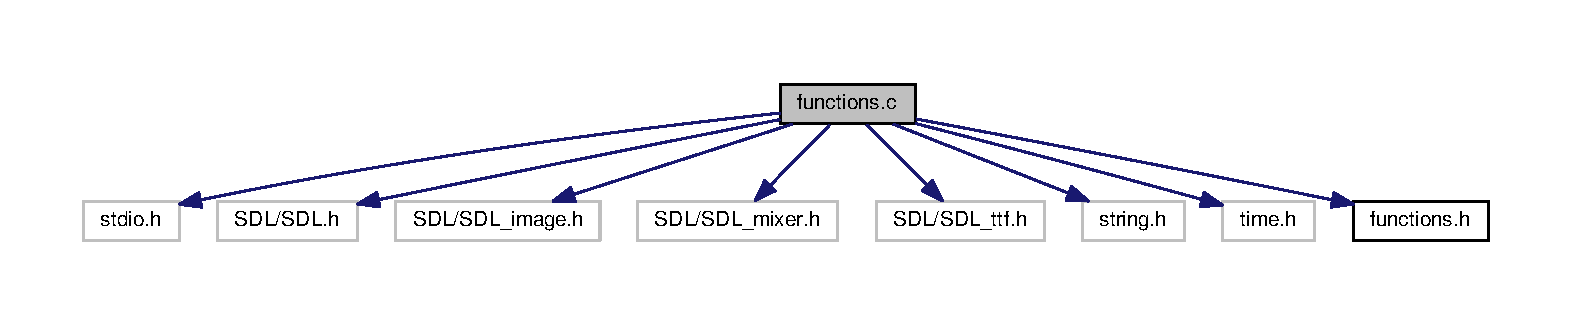
\includegraphics[width=350pt]{functions_8c__incl}
\end{center}
\end{figure}
\subsection*{Functions}
\begin{DoxyCompactItemize}
\item 
void {\bfseries initialiser} (F\+I\+LE $\ast$fichier, char $\ast$chaine, T\+T\+F\+\_\+\+Font $\ast$font, S\+D\+L\+\_\+\+Color color)\hypertarget{functions_8c_a5beb045907d5623923e9124da89ffc74}{}\label{functions_8c_a5beb045907d5623923e9124da89ffc74}

\item 
void {\bfseries generation} (S\+D\+L\+\_\+\+Surface $\ast$screen, S\+D\+L\+\_\+\+Surface $\ast$textbon, S\+D\+L\+\_\+\+Surface $\ast$textfaux, S\+D\+L\+\_\+\+Event event, S\+D\+L\+\_\+\+Rect position)\hypertarget{functions_8c_a4b26255e912d7ac838b6c7839919bdfc}{}\label{functions_8c_a4b26255e912d7ac838b6c7839919bdfc}

\item 
void {\bfseries choisir} (F\+I\+LE $\ast$fichier, T\+T\+F\+\_\+\+Font $\ast$font, S\+D\+L\+\_\+\+Color color, char $\ast$chaine, S\+D\+L\+\_\+\+Rect position)\hypertarget{functions_8c_a5f8a4043a3c02c18edb3355502c790f5}{}\label{functions_8c_a5f8a4043a3c02c18edb3355502c790f5}

\end{DoxyCompactItemize}

\hypertarget{functions_8h}{}\section{functions.\+h File Reference}
\label{functions_8h}\index{functions.\+h@{functions.\+h}}
This graph shows which files directly or indirectly include this file\+:\nopagebreak
\begin{figure}[H]
\begin{center}
\leavevmode
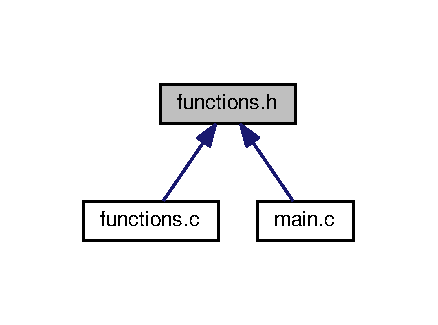
\includegraphics[width=210pt]{functions_8h__dep__incl}
\end{center}
\end{figure}
\subsection*{Functions}
\begin{DoxyCompactItemize}
\item 
void \hyperlink{functions_8h_a5beb045907d5623923e9124da89ffc74}{initialiser} (F\+I\+LE $\ast$fichier, char $\ast$chaine, T\+T\+F\+\_\+\+Font $\ast$font, S\+D\+L\+\_\+\+Color color)
\begin{DoxyCompactList}\small\item\em pour initialiser l\textquotesingle{}enigme \end{DoxyCompactList}\item 
void \hyperlink{functions_8h_a4b26255e912d7ac838b6c7839919bdfc}{generation} (S\+D\+L\+\_\+\+Surface $\ast$screen, S\+D\+L\+\_\+\+Surface $\ast$textbon, S\+D\+L\+\_\+\+Surface $\ast$textfaux, S\+D\+L\+\_\+\+Event event, S\+D\+L\+\_\+\+Rect position)
\begin{DoxyCompactList}\small\item\em pour generer la reponse (vrai/faux) \end{DoxyCompactList}\item 
void \hyperlink{functions_8h_a5f8a4043a3c02c18edb3355502c790f5}{choisir} (F\+I\+LE $\ast$fichier, T\+T\+F\+\_\+\+Font $\ast$font, S\+D\+L\+\_\+\+Color color, char $\ast$chaine, S\+D\+L\+\_\+\+Rect position)
\begin{DoxyCompactList}\small\item\em pour generer une question aleatoire a partir d\textquotesingle{}un fichier \end{DoxyCompactList}\end{DoxyCompactItemize}


\subsection{Function Documentation}
\index{functions.\+h@{functions.\+h}!choisir@{choisir}}
\index{choisir@{choisir}!functions.\+h@{functions.\+h}}
\subsubsection[{\texorpdfstring{choisir(\+F\+I\+L\+E $\ast$fichier, T\+T\+F\+\_\+\+Font $\ast$font, S\+D\+L\+\_\+\+Color color, char $\ast$chaine, S\+D\+L\+\_\+\+Rect position)}{choisir(FILE *fichier, TTF_Font *font, SDL_Color color, char *chaine, SDL_Rect position)}}]{\setlength{\rightskip}{0pt plus 5cm}void choisir (
\begin{DoxyParamCaption}
\item[{F\+I\+LE $\ast$}]{fichier, }
\item[{T\+T\+F\+\_\+\+Font $\ast$}]{font, }
\item[{S\+D\+L\+\_\+\+Color}]{color, }
\item[{char $\ast$}]{chaine, }
\item[{S\+D\+L\+\_\+\+Rect}]{position}
\end{DoxyParamCaption}
)}\hypertarget{functions_8h_a5f8a4043a3c02c18edb3355502c790f5}{}\label{functions_8h_a5f8a4043a3c02c18edb3355502c790f5}


pour generer une question aleatoire a partir d\textquotesingle{}un fichier 


\begin{DoxyParams}{Parameters}
{\em le} & fichier en question \\
\hline
{\em le} & font \\
\hline
{\em la} & couleur \\
\hline
{\em la} & chaine qui contiendra l\textquotesingle{}enigme \\
\hline
{\em la} & position \\
\hline
\end{DoxyParams}
\begin{DoxyReturn}{Returns}
rien 
\end{DoxyReturn}
\index{functions.\+h@{functions.\+h}!generation@{generation}}
\index{generation@{generation}!functions.\+h@{functions.\+h}}
\subsubsection[{\texorpdfstring{generation(\+S\+D\+L\+\_\+\+Surface $\ast$screen, S\+D\+L\+\_\+\+Surface $\ast$textbon, S\+D\+L\+\_\+\+Surface $\ast$textfaux, S\+D\+L\+\_\+\+Event event, S\+D\+L\+\_\+\+Rect position)}{generation(SDL_Surface *screen, SDL_Surface *textbon, SDL_Surface *textfaux, SDL_Event event, SDL_Rect position)}}]{\setlength{\rightskip}{0pt plus 5cm}void generation (
\begin{DoxyParamCaption}
\item[{S\+D\+L\+\_\+\+Surface $\ast$}]{screen, }
\item[{S\+D\+L\+\_\+\+Surface $\ast$}]{textbon, }
\item[{S\+D\+L\+\_\+\+Surface $\ast$}]{textfaux, }
\item[{S\+D\+L\+\_\+\+Event}]{event, }
\item[{S\+D\+L\+\_\+\+Rect}]{position}
\end{DoxyParamCaption}
)}\hypertarget{functions_8h_a4b26255e912d7ac838b6c7839919bdfc}{}\label{functions_8h_a4b26255e912d7ac838b6c7839919bdfc}


pour generer la reponse (vrai/faux) 


\begin{DoxyParams}{Parameters}
{\em l\textquotesingle{}ecran} & \\
\hline
{\em le} & text a generer si vrai \\
\hline
{\em le} & text a generer si faux \\
\hline
{\em l\textquotesingle{}evenement} & \\
\hline
{\em la} & position \\
\hline
\end{DoxyParams}
\begin{DoxyReturn}{Returns}
rien 
\end{DoxyReturn}
\index{functions.\+h@{functions.\+h}!initialiser@{initialiser}}
\index{initialiser@{initialiser}!functions.\+h@{functions.\+h}}
\subsubsection[{\texorpdfstring{initialiser(\+F\+I\+L\+E $\ast$fichier, char $\ast$chaine, T\+T\+F\+\_\+\+Font $\ast$font, S\+D\+L\+\_\+\+Color color)}{initialiser(FILE *fichier, char *chaine, TTF_Font *font, SDL_Color color)}}]{\setlength{\rightskip}{0pt plus 5cm}void initialiser (
\begin{DoxyParamCaption}
\item[{F\+I\+LE $\ast$}]{fichier, }
\item[{char $\ast$}]{chaine, }
\item[{T\+T\+F\+\_\+\+Font $\ast$}]{font, }
\item[{S\+D\+L\+\_\+\+Color}]{color}
\end{DoxyParamCaption}
)}\hypertarget{functions_8h_a5beb045907d5623923e9124da89ffc74}{}\label{functions_8h_a5beb045907d5623923e9124da89ffc74}


pour initialiser l\textquotesingle{}enigme 


\begin{DoxyParams}{Parameters}
{\em le} & fichier contenant l\textquotesingle{}enigme \\
\hline
{\em la} & chaine qui recevra l\textquotesingle{}enigme \\
\hline
{\em le} & font a utiliser \\
\hline
{\em la} & couleur a utiliser \\
\hline
\end{DoxyParams}
\begin{DoxyReturn}{Returns}
rien 
\end{DoxyReturn}

\hypertarget{main_8c}{}\section{main.\+c File Reference}
\label{main_8c}\index{main.\+c@{main.\+c}}


prog test  


{\ttfamily \#include $<$stdio.\+h$>$}\\*
{\ttfamily \#include \char`\"{}S\+D\+L/\+S\+D\+L.\+h\char`\"{}}\\*
{\ttfamily \#include \char`\"{}S\+D\+L/\+S\+D\+L\+\_\+image.\+h\char`\"{}}\\*
{\ttfamily \#include \char`\"{}S\+D\+L/\+S\+D\+L\+\_\+mixer.\+h\char`\"{}}\\*
{\ttfamily \#include \char`\"{}S\+D\+L2/\+S\+D\+L\+\_\+rotozoom.\+h\char`\"{}}\\*
Include dependency graph for main.\+c\+:

%--- End generated contents ---

% Index
\backmatter
\newpage
\phantomsection
\clearemptydoublepage
\addcontentsline{toc}{chapter}{Index}
\printindex

\end{document}
